%% This is an example first chapter.  You should put chapter/appendix that you
%% write into a separate file, and add a line \include{yourfilename} to
%% main.tex, where `yourfilename.tex' is the name of the chapter/appendix file.
%% You can process specific files by typing their names in at the
%% \files=
%% prompt when you run the file main.tex through LaTeX.
\chapter{Experience and Outcomes
}
The purpose of this chapter is to investigate how past experience affect current outcomes in the market for public construction projects. Section 1 outlines the empirical strategy, .

\section{Data}
Recall that our dataset consist in a set of bids submitted by firms in first-price, sealed bid auctions developed by the government in Chile between 2010 and 2020 for construction projects. The source and main characteristics of the dataset employed in the investigation were detailed in the previous section. Now we detail the specifics of the subset employed for the current sresearch question.

 We further filter the dataset in the following way. we only consider contracts with and estimated price above 20.000.000 CLP to exclude extremely simple contracts, and proposals below 10.000.000 CLP as well. We also excluded contracts without an official estimate. We exclude non-single-item proposals. Finally, we exclude contracts with several proposals from a given contractor as we have no clear way of distinguisinh which was the last submitted one.

As a result of the previous filtering steps we end with around 43,000 construction contracts, of the original sample of about 74,000 contracts. We excluded around 5\% of the original sample which had no  official estimate(which are excluded), and around 2\% which are not single-item proposals. By far the most important filtering step is excluding contracts with estimated values of less than 20.000.000 CLP, which excludes around 41\% of the original dataset (around 30,000 contracts). Finally, around a 1,200 contracts had multiple proposals from the same contractor. Note that some of the previous conditions overlapped among them.

The table shows descriptive statistics for the final sample employed.
\begin{table}[!h]

\caption{Descriptive Statistics}
\centering
\resizebox{\textwidth}{!}{
\begin{tabular}[t]{cccccc}
\toprule
name & N & mean & std & max & min\\
\midrule
Bid (all) & 119000 & 1.73e+10 & 5.8e+12 & 2e+15 & 1e+07\\
Winning Bid & 32200 & 2.27e+08 & 2.54e+09 & 2.47e+11 & 1e+07\\
Difference between 1st bid and 2nd (\%) & 32200 & 0.0638 & 0.0859 & 0.984 & 0\\
Number of Bidders per Contract & 32200 & 3.18 & 2.25 & 23 & 1\\
Year & 32200 & 2020 & 2.89 & 2020 & 2010\\
Offers made by Firm & 13800 & 8.64 & 18.5 & 846 & 1\\
Win prob. by Firm & 13800 & 0.213 & 0.294 & 1 & 0\\
Offers won by Firm & 13800 & 2.33 & 5.66 & 111 & 0\\
\bottomrule
\end{tabular}
}
\vskip 0.5mm
{\raggedright \footnotesize \underline{Note:} The table shows sample summary statistics for the public construction dataset after filtering has been applied (see text). The difference between 1st(winning) and 2nd (runner-up) bid is only avalaible in approx. 70\% od the contracts, with two or more bidders. \par}
\end{table}



\section{Empirical Strategy}
Our empirical strategy consists in a Regression Discontinuity design in which we compare the bidding outcomes of firms with varying degrees of previous experience in the market. Our main interest is the difference between the firms with some and the firms with none experience, but we consider also increasing measures of experience.

Our main outcome variable is the share of contracts won out of the total amount of contracts bid for, in a specific period of time. That is, if we consider period $t$, then the outcome variable for firm $i$ is $\dfrac{W_{it}}{B_{it}}$ where $B_{it}$ are the bids submitted by firm $i$ on the period $[t,t+\tau]$, $W_{it}$ are the contracts won in period $[t,t+\tau]$ and $\tau$ is a reasonable parameter which controls the duration of the periods i which we compute both experience and outcomes. In our initial specification, we consider each $tau$ to be equal to two years, and each $t$ is the first day of the year in our dataset. Employing a proportion of contracts won instead of total contracts has two advantages. First, we implicitly control by size. Second, we can capture directly the impact of firms which bid in contracts with no competitors.

%Our dependent variable is a measure of firms' past experience. In #principle, there are several ways in which we could measure experience. We could employ, for example, the total amount of dollars executed up until one point in time or the number of contracts won. We employ the latter to better capture the discrete differences occurring between zero and more than zero contracts performed in past periods. In our specifications, we consider experience binary indicator of past experience, a linear polynomial and also second-degree polynomial.

Regarding the measurement of experience for a given firm and period, we consider two main options. The first one is to consider experience as the total amount of contracts won in a fixed period before the period of outcomes being considered. The second alternative we consider is a rolling average of yearly contracts developed up until that same period of outcomes. The robustness checks consider also other measures of experience.

The first option is implemented as follows. We create a dataset where observations are period-firm pairs and variables are measures of past experience and current outcomes in the following way. We fix a specific start date and an end date to define a first period (Period 1), which is used to compute the experiences of each firm. Then, for each firm we link this experience to the outcomes in a subsequent period of equal length (Period 2).  This way, we construct a dataset where each observation is a firm, the dependent variable is a measure the firm’s outcome in Period 2, and the independent variables is a measure of the (past) experience of the firm in Period 1. We repeat this process, considering as Period 1 successive two-year periods in our dataset with one year of overlap between them. Since our dataset contains 10 years, we end up with four two-year pairs (we do not have outcomes for the last two years in our data).

A key parameter in this strategy is the length in years of period 1 and period 2. They are arbitrary and could be differ from each other. As our baseline, we employ two-years periods for the following reasons. First, we do not expect that an active firm will spend more than one year without bidding. Our full dataset shows that for every firm on the data who bid having previous experience, a 50\% has developed a contract within the last 2 years. Second, we do not want to employ too long periods as that would confound the effect of experience for early-period entrants. However, periods of one or three years could be reasonable as well, so we relax this assumption in the robustness checks and experiment with a wider array of periods’ lengths.

For the second alternative to measure experience we construct an annualized measure of experience in the following way. Our success periods are constructed in the same way as before. However, instead of restricting our measure of past experience to two years before the beginning of the period, we consider all the previous periods to count contracts won. In order to obtain comparable estimates across successive years, for each period we divide the total contracts developed by the firm up until that moment by the number of years where we are considering experience. This way, we obtain an “annualized” measure of experience.

Our two main specification are of the following form, where $S_{it }$ is the share of contracts won in the period of interest, $EXP_{it} $ is the measure of experience of firm $i$ in period $t-1$ or up until $t$(depending on the specification), and $T_t$ are period fixed effect.

$$S_{it}=\alpha+ \beta EXP_{it-1}+T_t$$

In some specifications we include firm fixed effects based on size. It is possible that smaller firms face higher competition due to less-complex contracts, and so their baseline level of success in the market will be lower. Additionally, we add period  fixed effects for each period of outcomes being considered to control for changes in the market environment throughout the sample.

\subsection{Endogeneity and Identification}
Causal interpretation of the regression above is problematic since unobserved cost variables are endogenous. It would be expected that highly efficient firms are able to bid more aggressively, win more projects, and in turn accrue more experience in the market of public construction projects. In the base case, we expect our estimates of the effect of experience on outcomes to be biased upwards due to unobserved cost variables which should have positive correlation with experience.

In order to identify the causal experience of experience on outcomes, we employ external variation in the experience of a firm. We employ as the main source of identification the exogenous variation produced by close wins, which should be less or not at all attributed to unobserved cost factors. We arbitrarily define a win as a close win if the percentage difference between the winner and the runner-up is less than 0.5\%. This leads to approximately 8\% of winning bids being classified as a close one.  In the robustness checks, we also consider a different approach to close wins, where we consider close wins where three or more competitors are all within a 1\% difference in their bids.

In the next table we examine whether close wins are different from the population in several types of metrics. We can see that in most aspects these bids are not exceedingly different from the rest of the sample, so we expect that the only difference between these close wins and regular ones is the difference in bids and there are no underlying project characteristics that could explain them.

\begin{table}[!h]
\caption{Comparison of key statistics between close wins(<0.05\% difference between 1st and runner-up) and regular wins}
\centering
\resizebox{\textwidth}{!}{
\begin{tabular}[t]{ccccc}
\toprule
Variable & Mean (Not close win) & Mean (Close win) & Sd (Not close win) & Sd (Close win)\\
\midrule
Bid & 6.3e+08 & 3.32e+10 & 1.06e+10 & 8.11e+12\\
Bid\_Winning & 3.18e+08 & 2.37e+08 & 3.56e+09 & 2.62e+09\\
Difference between 1st bid and 2nd (\%) & 0.14 & 0.0186 & 0.115 & 0.0147\\
Number of Bidders & 3.86 & 4.08 & 2.12 & 2.23\\
Year & 2020 & 2020 & 2.92 & 2.89\\
Offers made by Firm & 4.4 & 6.17 & 7.34 & 11.2\\
Win prob. by Firm & 0.191 & 0.171 & 0.3 & 0.274\\
Offers won by Firm & 0.972 & 1.37 & 2.1 & 3.23\\
\bottomrule
\end{tabular}
}
\end{table}

Our designs employs close wins in past periods to instrument total wins (experience). Clearly, both measures are correlated since every extra unit of experience increases the probability of having at least one close win. Moreover, close wins should not be correlated with cost measures, as they are attributed to random factors, such as risk-aversion differences between firms, random approximation differences between engineering teams in each firm, etc. and thus we should also have a valid instrument.


%Bidding behavior
%An alternative way to measure changes in bidding behavior caused by efficiency gains through experience is to examine directly changes in bidding behavior among more experienced firms with respect to less experienced ones. As was discussed before, experience induces changes in the underlying production function, or changes along the production function, that make the firm more efficient at producing certain types of goods. In a competitive market, firms should pass through at least a fraction of this improvement in costs to the bids they submit in the auctions. Thus, we should be able to identify this change directly through the bids that more experienced firms submit for projects.
%The approach is different than the one from the previous section because we can directly link the past experience of a firm to each bid it submits in every auction that it participates in. Thus, our unit of observation is a bid submitted by a firm for a contract of a public construction contract. Our second specification has then the following form:where is the standardized bid submitted by the firm and is a measure of past experience. In further specifications we include a broader set of controls. First, we add fixed effects by auction. Second, we add firm fixed effects. Finally, we control by the geographic region where the auction is being held.
%The outcome variable is the standardized bid submitted by firm to the auction, i.e. the original bid amount divided by the engineering estimate of the project. This approach allows us to make comparisons along project of different sizes. It is also useful because it should be expected that our dependent variables have effects per unit of contract amount (Bajari, 2010). The standardization also controls for some sources of heterogeneity.
%The dependent variable is the total number of contracts that the firm has won up until the moment that the firm submits its bid. Since for the first periods in the data we do not have information on past experience, we exclude the first two years from our observations of outcomes and only employ them to compute experiences for firms from year three and onward. In the robustness section, we explore several alternative ways to measure experience and subset the set of firms.
%In the same way as before, we expect that there will an endogeneity between cost measures and bidding behavior. We should expect that firms which have a baseline efficiency higher than other firms will be able to submit lower bids and gain more experience, so we could pick up effects of reverse causation in our coefficient for experience.  We thus employ a similar Instrumental Variables approach as before, instrumenting total past contract wins with close contract wins.

\section{Main Results}

First we explore graphically the relationship between experience and outcomes. Figure \ref{fig:plotresults_both} , Panel A, shows the relationship between experience and outcomes for firms. While we can see an increase in the average share of contracts won, the sample contains heteregeneity, as per the wide error bars(which show interquartile range). Panel B contains only two types of firms: firms that either bid but not won contracts in period $(t-1)$ or firms which won one or more close contracts in period $t$.

\begin{figure}
  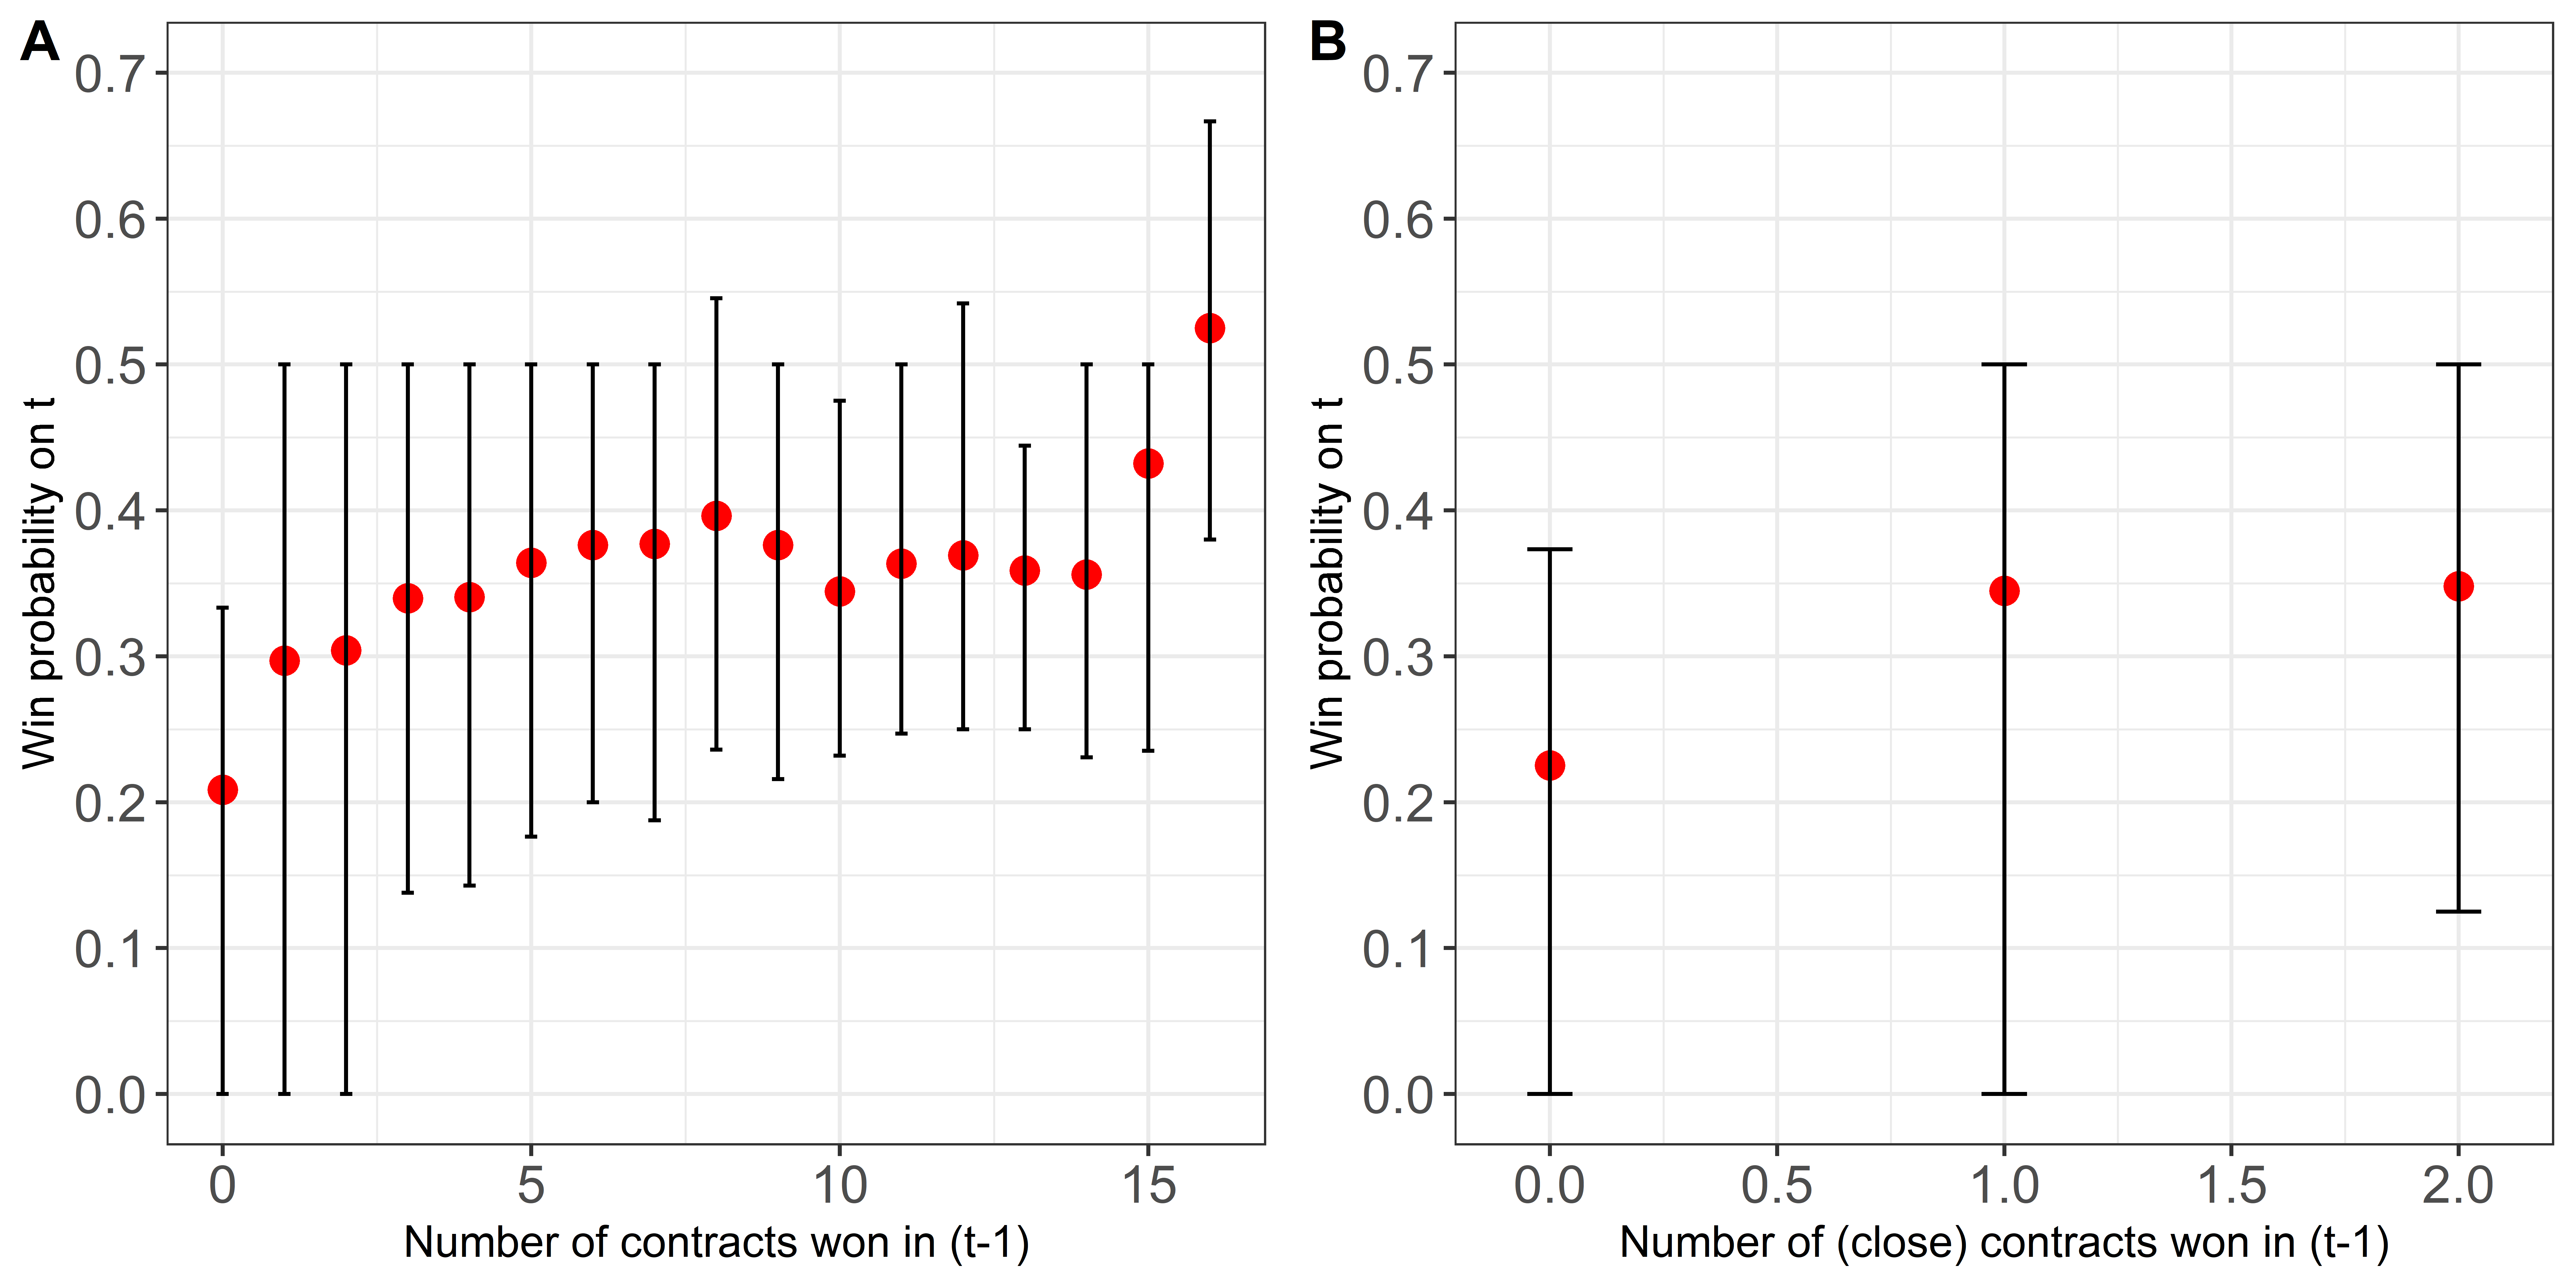
\includegraphics[scale=0.65]{plotwins_both.png}
  \caption{Relationship between contracts won on $t-1$ and mean winning probability across contractors in $t$.}
  \label{fig:plotresults_both}
  \vskip 0.5mm
  { \footnotesize \underline{Note:} The plots show the mean across firms of the number of contracts won out of the number of contracts bid for in period $t$ (in the $y$-axis), against experience accrued in period $(t-1)$ in the $x$-axis. $t$ and $t-1$ correspond to two periods of two years each. Since the data contains ten years, the observations correspond to outcomes computed for eight outcome periods.  Only $x$ for which the number of observations is greater than ten are shown. Error bars correspond to the interquartile range. Panel A: all sample observations are considered. Panel B:  shows results for a subsample where the only contractors considered are those who either i) won closely one or more close contracts  on period 1 or ii) did bid but not win a contract in period 1\par}
\end{figure}

Table \ref{table1} shows the results for specifications with the reduced form regression and IV estimates for our first Experience computation measure (i.e. rolling two year periods) while Table \ref{tableExp2} shows the results for our way of computing experience (i.e. total annualized experience).

In both tables, OLS results are in the first to third panels. The first panel shows that the OLS coefficient on the effect of having experience against not having experience (binary) is around 0.10, for both ways of computing experience. Our specification with linear returns on experience shows that experience renders a 0.02 and 0.05 increase in winning share per extra contract developed (for computations 1 and 2 respectively) . All the estimates for the experience-related coefficients are significant at 0.01 with robust standard errors.

The IV results (fourth to sixth panels in each table) show that  the linear and quadratic estimates of the coefficients on experince generally stay within $\pm$ 0.03 of their OLS counterparts. There is however an increase in the binary measure of experience coefficient, for both computations of experience.

A concerning result is the low $R^2$, which shows that altough the effect of experience on the mean outcome is significant, there is much variability among firms which is not accounted by experience. This points towards a market more competitive than was originally hypothesized.

\begin{table}[!htbp] \centering
  \caption{Regression results for OLS and IV specifications where experience is computed in 2-year rolling periods}
  \label{tab:table_exp_1}
  \resizebox{\textwidth}{!}{
  \begin{tabular}{@{\extracolsep{5pt}}lcccccc}
  \\[-1.8ex]\hline
  \hline \\[-1.8ex]
   & \multicolumn{6}{c}{\textit{Dependent variable:}} \\
  \cline{2-7}
  \\[-1.8ex] & \multicolumn{6}{c}{Share of Contracts won in t} \\
  \\[-1.8ex] & \multicolumn{3}{c}{\textit{OLS}} & \multicolumn{3}{c}{\textit{instrumental}} \\
   & \multicolumn{3}{c}{\textit{}} & \multicolumn{3}{c}{\textit{variable}} \\
  \\[-1.8ex] & (1) & (2) & (3) & (4) & (5) & (6)\\
  \hline \\[-1.8ex]
   Experience in (t-1) (Binary) & 0.119$^{***}$ &  &  & 0.178$^{***}$ &  &  \\
    & (0.004) &  &  & (0.010) &  &  \\
    & & & & & & \\
   Experience in (t-1) (Linear) &  & 0.022$^{***}$ & 0.038$^{***}$ &  & 0.022$^{***}$ & 0.039$^{***}$ \\
    &  & (0.002) & (0.001) &  & (0.001) & (0.003) \\
    & & & & & & \\
   (Experience in (t-1)) (Squared) &  &  & $-$0.001$^{***}$ &  &  & $-$0.001$^{***}$ \\
    &  &  & (0.0001) &  &  & (0.0003) \\
    & & & & & & \\
   Constant & 0.260$^{***}$ & 0.276$^{***}$ & 0.270$^{***}$ & 0.245$^{***}$ & 0.276$^{***}$ & 0.269$^{***}$ \\
    & (0.005) & (0.005) & (0.005) & (0.005) & (0.005) & (0.005) \\
    & & & & & & \\
  \hline \\[-1.8ex]
  Fixed effects By period & Yes & Yes & Yes & Yes & Yes & Yes \\
  Observations & 37,959 & 37,959 & 37,959 & 37,959 & 37,959 & 37,959 \\
  R$^{2}$ & 0.035 & 0.028 & 0.034 & 0.028 & 0.028 & 0.034 \\
  Residual Std. Error & 0.316 (df = 37950) & 0.317 (df = 37950) & 0.316 (df = 37949) & 0.317 (df = 37950) & 0.317 (df = 37950) & 0.316 (df = 37949) \\
  \hline
  \hline \\[-1.8ex]
  \textit{Note:}  & \multicolumn{6}{r}{$^{*}$p$<$0.1; $^{**}$p$<$0.05; $^{***}$p$<$0.01} \\
  \end{tabular}

}

\end{table}

The next table shows the  results with a different measure of experience.
\begin{table}[!htbp] \centering
  \caption{Regression results for OLS and IV specifications where experience is computed as past annualized contracts won.}
  \label{tableExp2}
  \resizebox{\textwidth}{!}{
  \begin{tabular}{@{\extracolsep{5pt}}lcccccc}
  \\[-1.8ex]\hline
  \hline \\[-1.8ex]
   & \multicolumn{6}{c}{\textit{Dependent variable:}} \\
  \cline{2-7}
  \\[-1.8ex] & \multicolumn{6}{c}{Share of Contracts won in t} \\
  \\[-1.8ex] & \multicolumn{3}{c}{\textit{OLS}} & \multicolumn{3}{c}{\textit{instrumental}} \\
   & \multicolumn{3}{c}{\textit{}} & \multicolumn{3}{c}{\textit{variable}} \\
  \\[-1.8ex] & (1) & (2) & (3) & (4) & (5) & (6)\\
  \hline \\[-1.8ex]
   Experience in (t-1) (Binary) & 0.109$^{***}$ &  &  & 0.168$^{***}$ &  &  \\
    & (0.004) &  &  & (0.010) &  &  \\
    & & & & & & \\
   Experience in (t-1) (Linear) &  & 0.059$^{***}$ & 0.107$^{***}$ &  & 0.057$^{***}$ & 0.108$^{***}$ \\
    &  & (0.016) & (0.004) &  & (0.004) & (0.012) \\
    & & & & & & \\
   (Experience in (t-1)) (Squared) &  &  & $-$0.013$^{***}$ &  &  & $-$0.013$^{***}$ \\
    &  &  & (0.001) &  &  & (0.003) \\
    & & & & & & \\
   Constant & 0.288$^{***}$ & 0.289$^{***}$ & 0.285$^{***}$ & 0.277$^{***}$ & 0.290$^{***}$ & 0.285$^{***}$ \\
    & (0.005) & (0.006) & (0.005) & (0.006) & (0.005) & (0.005) \\
    & & & & & & \\
  \hline \\[-1.8ex]
  Fixed effects By period & Yes & Yes & Yes & Yes & Yes & Yes \\
  Observations & 36,844 & 36,844 & 36,844 & 36,844 & 36,844 & 36,844 \\
  R$^{2}$ & 0.032 & 0.027 & 0.031 & 0.025 & 0.027 & 0.031 \\
  Residual Std. Error & 0.321 (df = 36835) & 0.322 (df = 36835) & 0.321 (df = 36834) & 0.322 (df = 36835) & 0.322 (df = 36835) & 0.321 (df = 36834) \\
  \hline
  \hline \\[-1.8ex]
  \textit{Note:}  & \multicolumn{6}{r}{$^{*}$p$<$0.1; $^{**}$p$<$0.05; $^{***}$p$<$0.01} \\
  \end{tabular}

}

\end{table}


There does not seems to be conclusive evidence regarding different results when employing quadratic rather than linear functional forms. For example, Figure \ref{fig:fit_sample} shows the mean confidence intervals, employing as period fixed effects the last period in the sample. It can be seen that the fitted total predicted value does not seen to vary greatly from the linear to the quadratic specification.

\begin{figure}[H]
        \centering
        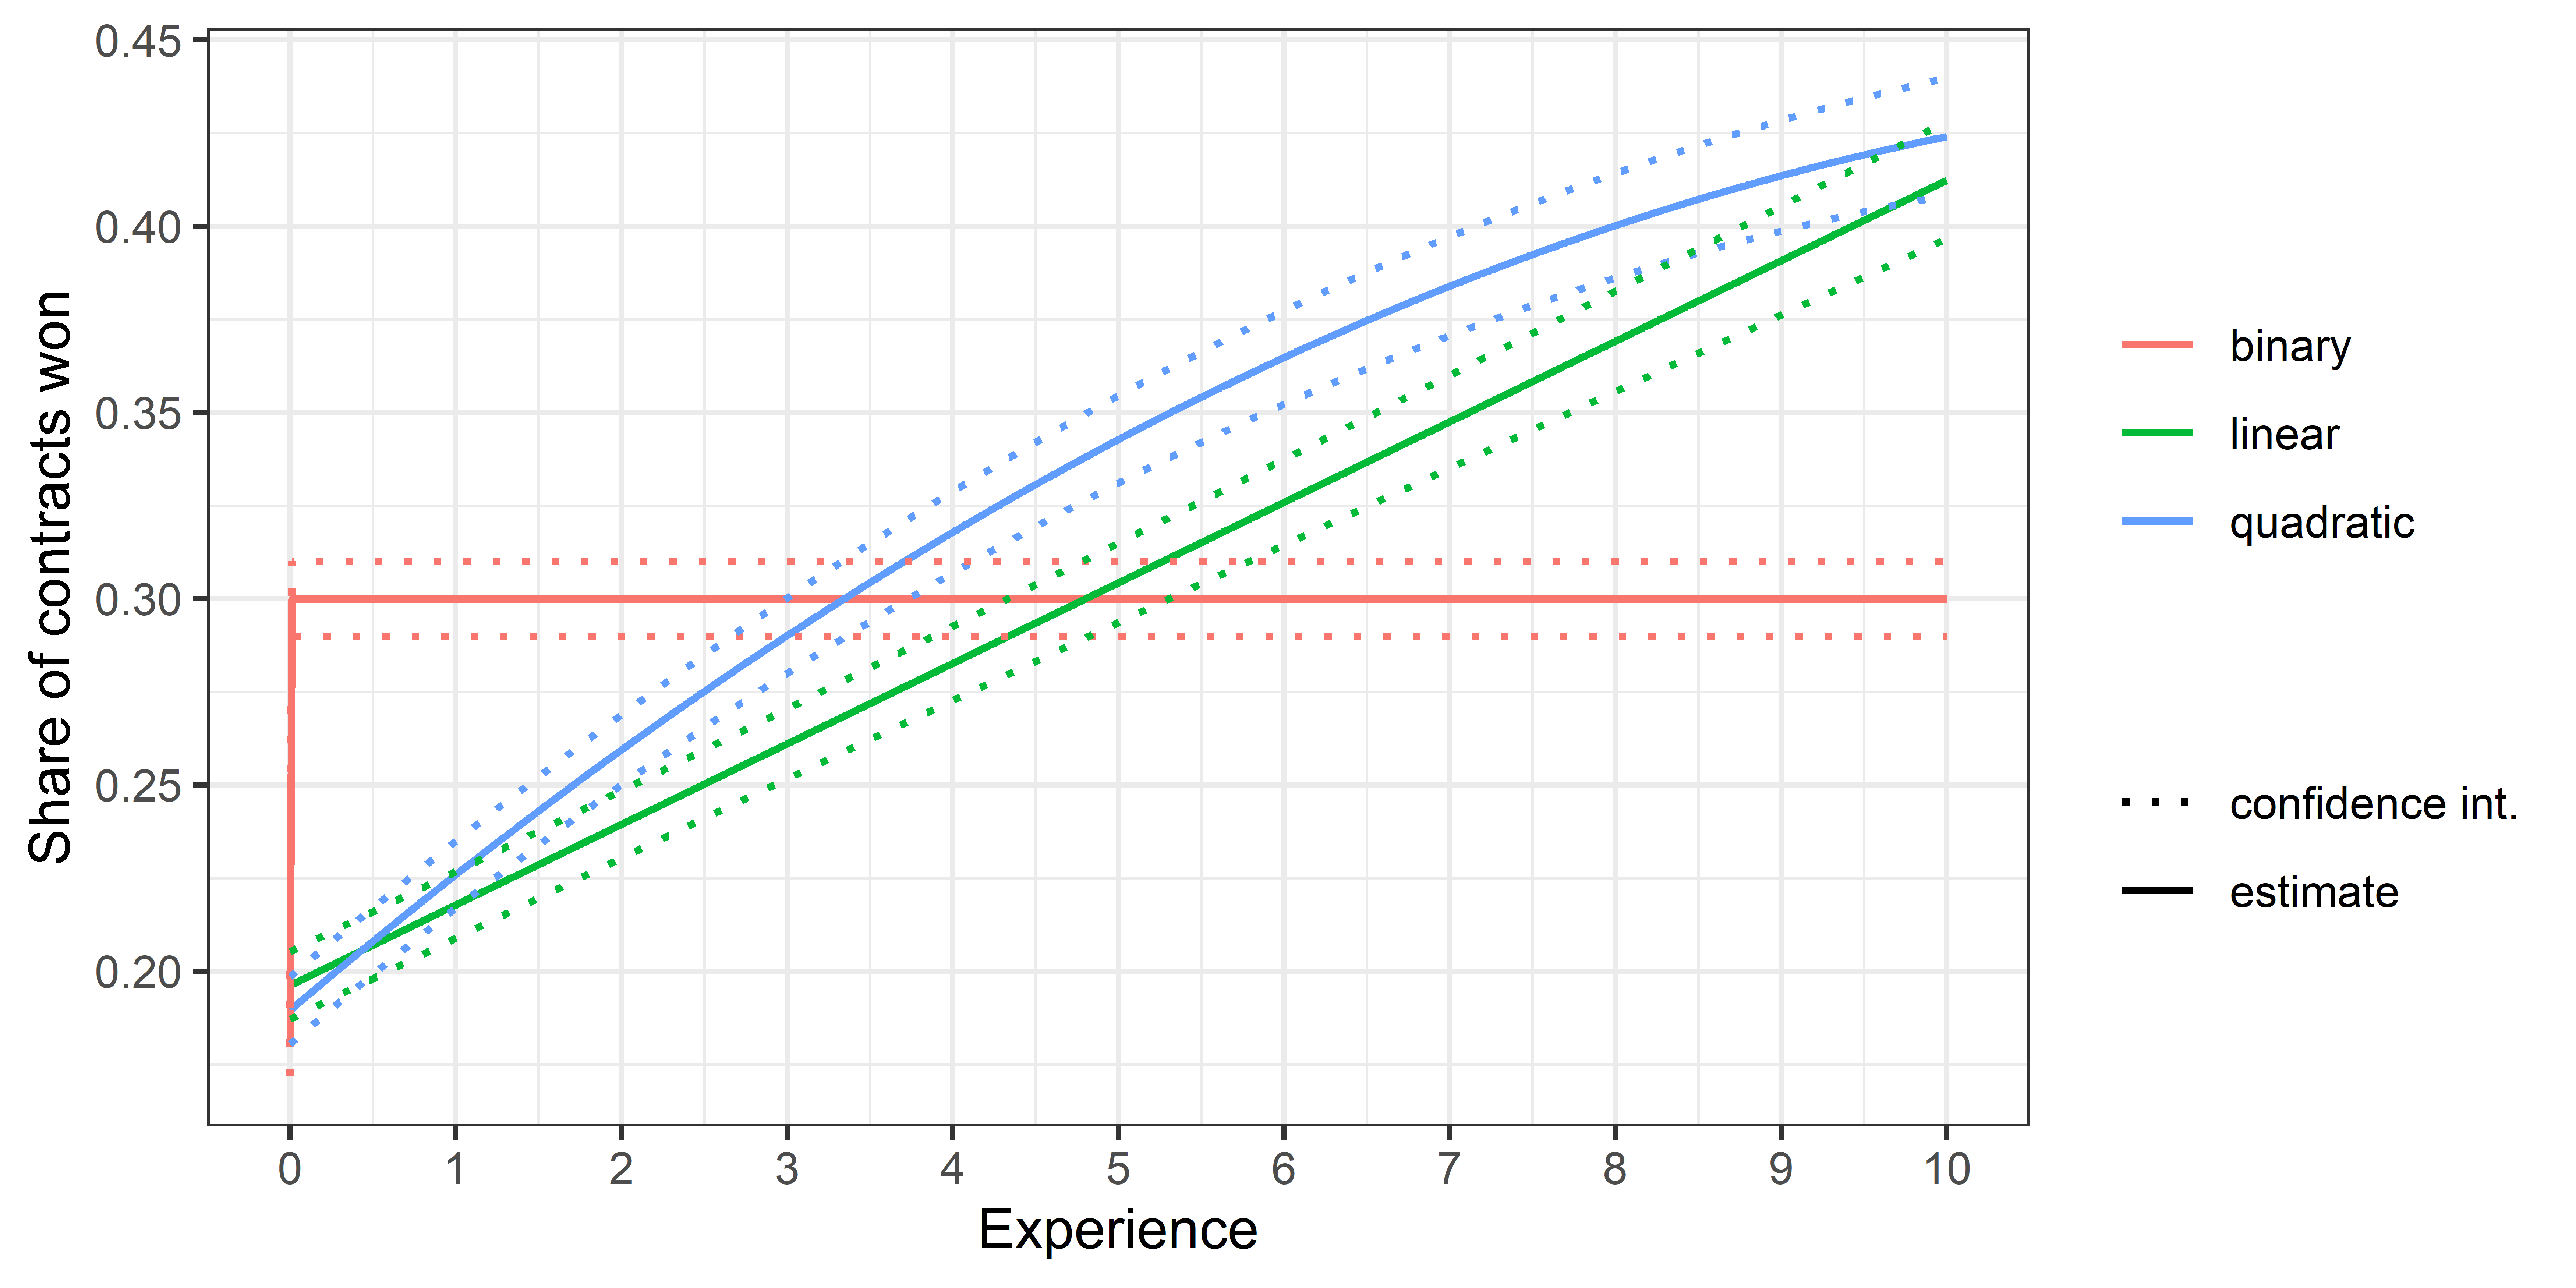
\includegraphics[scale=0.8]{fit_sample.png}
        \caption{ \small Predicted values for the mean of the outcome variable (share of contracts won), by total experience accrued in the previous period. We employ fixed effects as in the last period of the dataset.}
        \label{fig:fit_sample}
    \end{figure}




\section{Experience and Type of Project}
Given our previous results a natural concern is if whether all projects exhibits the same returns to experience or if experience is more important in certain types of works. In this section we replicate the previous analysis by disaggregating by type of project. In order to do this, we classify certain projects according to their description, then run similar regressions as in the last section, and present the results.

First we describe briefly how we construct categories for the prrojects and which ones are avalaible for the analysis. Our original dataset includes a name variable which describes the type of project with some extent. We extracted this name variable and looked for i) common single words (unigrams) and ii) common pairs of words (bigrams). We select the most common unigrams and bigrams and map similar words and bigrams to project categories. The full categorization mapping can be found in the Appendix.

We end up with contract classified under categories. Importantly, if a contract includes unigrams or bigrams in its name belonging to more than one category, it is included in the analysis of both categories. The number of contracts, average amount, average number of bidders for each category is shown in Table \ref{}. We can see that the biggest categories of projects are school-related, vecinal works, parks and pavements (including sidewalks). The Appendix contains more details on the types of projects included in each category.

%\input{C:/repos/learn-doing/thesis/tables/table_types_project_stats.txt}

Next we run similar regressions as in the previous section for each project type, considering as our dataset only the contracts in that project category . We employ the same specification of with a linear functional form on experience and period fixed effects, and our first measure of experience. The results are presente in Figure \ref{fig:typeestimates}he Appendix includes more detailed tables with full regression results for each sproject type. A few results stand out. First, we get the biggest coefficients on experience on graveyard projects, footbridges and housing. The first two should be almost exclusively procured by government units. Housing was also one of our hypothsized types of projects which should have high coefficients. At the bottom of the distribution, interestingly, we find daycares, sports courts, hospitals, and schools. The results could be explained because these projects are mostly composed of normal construction works which also have private close substitutes.

The results on hospitals should be surprising, as they are usually very big projects with a lot of specific knwoledge required.

%\input{C:/repos/learn-doing/thesis/tables/table_types_project_ols.txt}

\begin{figure}
  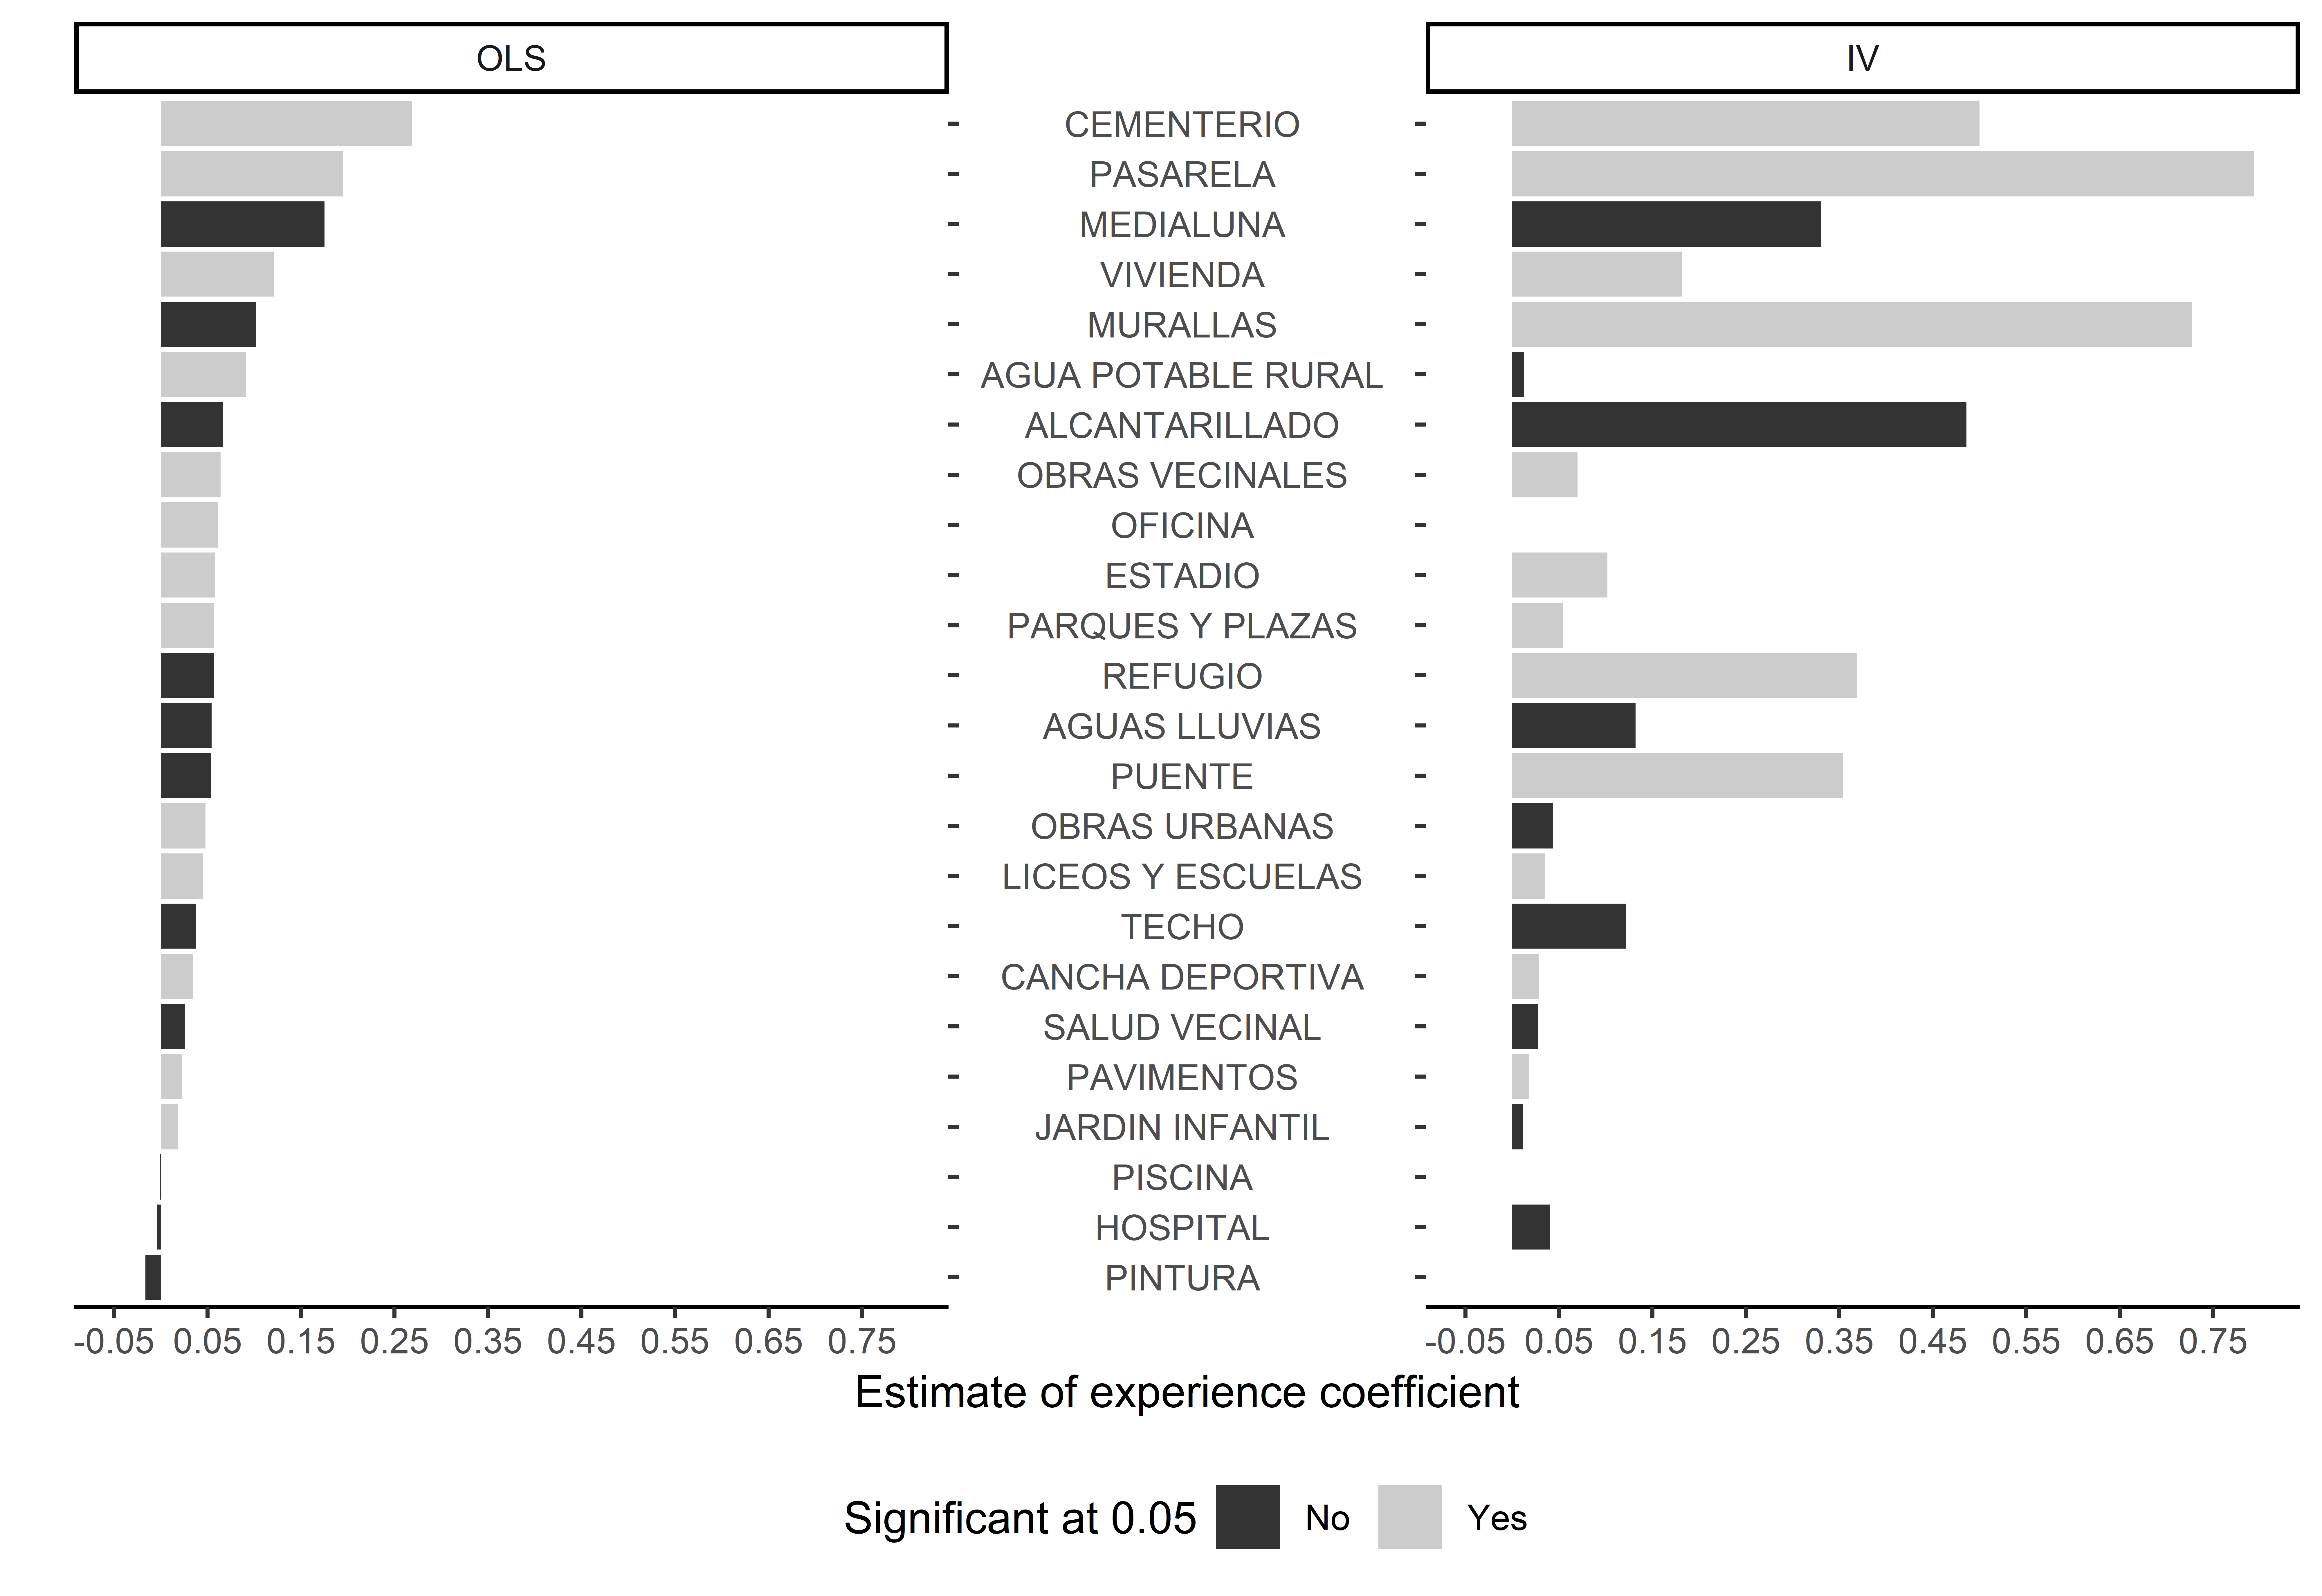
\includegraphics[scale=0.75]{plotTypes.png}
  \caption{Experience coefficient by type of project.}
  \label{fig:typeestimates}
\end{figure}

\section{Experience and Firm Size}
%In the literature about industrial organization and productivity, it has been studied the relation between firm size, innovation, and productivity. These investigations have concluded that smaller firms are more productive than bigger firms, however they are also more risky.
An important variable in the investigation of the effect of experience should be firm size. First, it is possible that there are different levels of cost efficiency between small and big firms. As arguably bigger firms should have more experience on average, this could skew our estimates. A second concern is that we might expect experience to matter more for smaller firms, if there is a decreasing or "maximum" level effect of experience on future outcomes.

If our identification strategy is correct, firm size should not be a problem for the reliability of the estimates obtained in the previous section, while the effect of experience by size is still unclear. In this section we attempt to develop specific estimates of the effect of experience for different levels of firm size. Developing intra-category estimates serves as both as an identification strategy and as  robustness check of our previous findings.

 We follow the following approach. First we select a subsample from our original dataset which we can classify acoording to annual sales.  We obtain intra-category estimates of the effect of experience and interpret them. Finally, we discuss the results and some of the empirical challenges of controlling for size.

In order to study and control for firm size we employ a publicily avalaible classification of firms according to their annual sales, maintained by the chilenan Tax Bureau Office (\textit{Servicio de Impuestos Internos}). Firms are categorized in 13 categories. Category number one  corresponds to 'tax data not enough to classify', but from catoegory two upo to thirteen, each category is defined by an increasing level of minimum yearly sales.  However, this data is avalaible only for non-individual firms. After merging with our initial sample,we are left with around 30\% of our original firm sample. Table \ref{tab:salescategories} shows how many firms do we have in our sample for each category, average annual sales for these firms, and statutory annual sales thresholds for each category. Note that we have much more firms at intermediate categories than extreme ones.

% Table generated by script
\input{C:/repos/learn-doing/thesis/tables/table_tax_categories_data.txt}

We estimate the effect of linear experience with our first measure for each category of firms by OLS and IV. Specifications are the same as equation with period fixed effects. The results are presented graphically in \ref{fig:sizeestimates} (the coefficient for category two is omitted because it was much bigger than the rest and distorted the visualiztion). Full results are avalaible at the Appendix.

We only obtain significant effects at intermediate sales categories' levels. However, everytime a coefficient is significant it is also positive. The results are not supreising given i) the reduced sample we are employing ii) the expected reduced importance of experience for very big firms.

Controlling for firm size is challenging mainly because of statistical reasons. First, firm size distribution in the sample is not uniform as there are less very small and very big firms. Second, the within-size distribution of experience within extreme categories has very few observations with more than five contracts of experience. Third, this sample is already smaller due to filtering single-person companies. Both factors make it hard to obtain per-category estimates with enough statistical power experience.

\newpage
\input{C:/repos/learn-doing/thesis/tables/table_firm_sizes_intercepts.txt}


%\begin{figure}
%  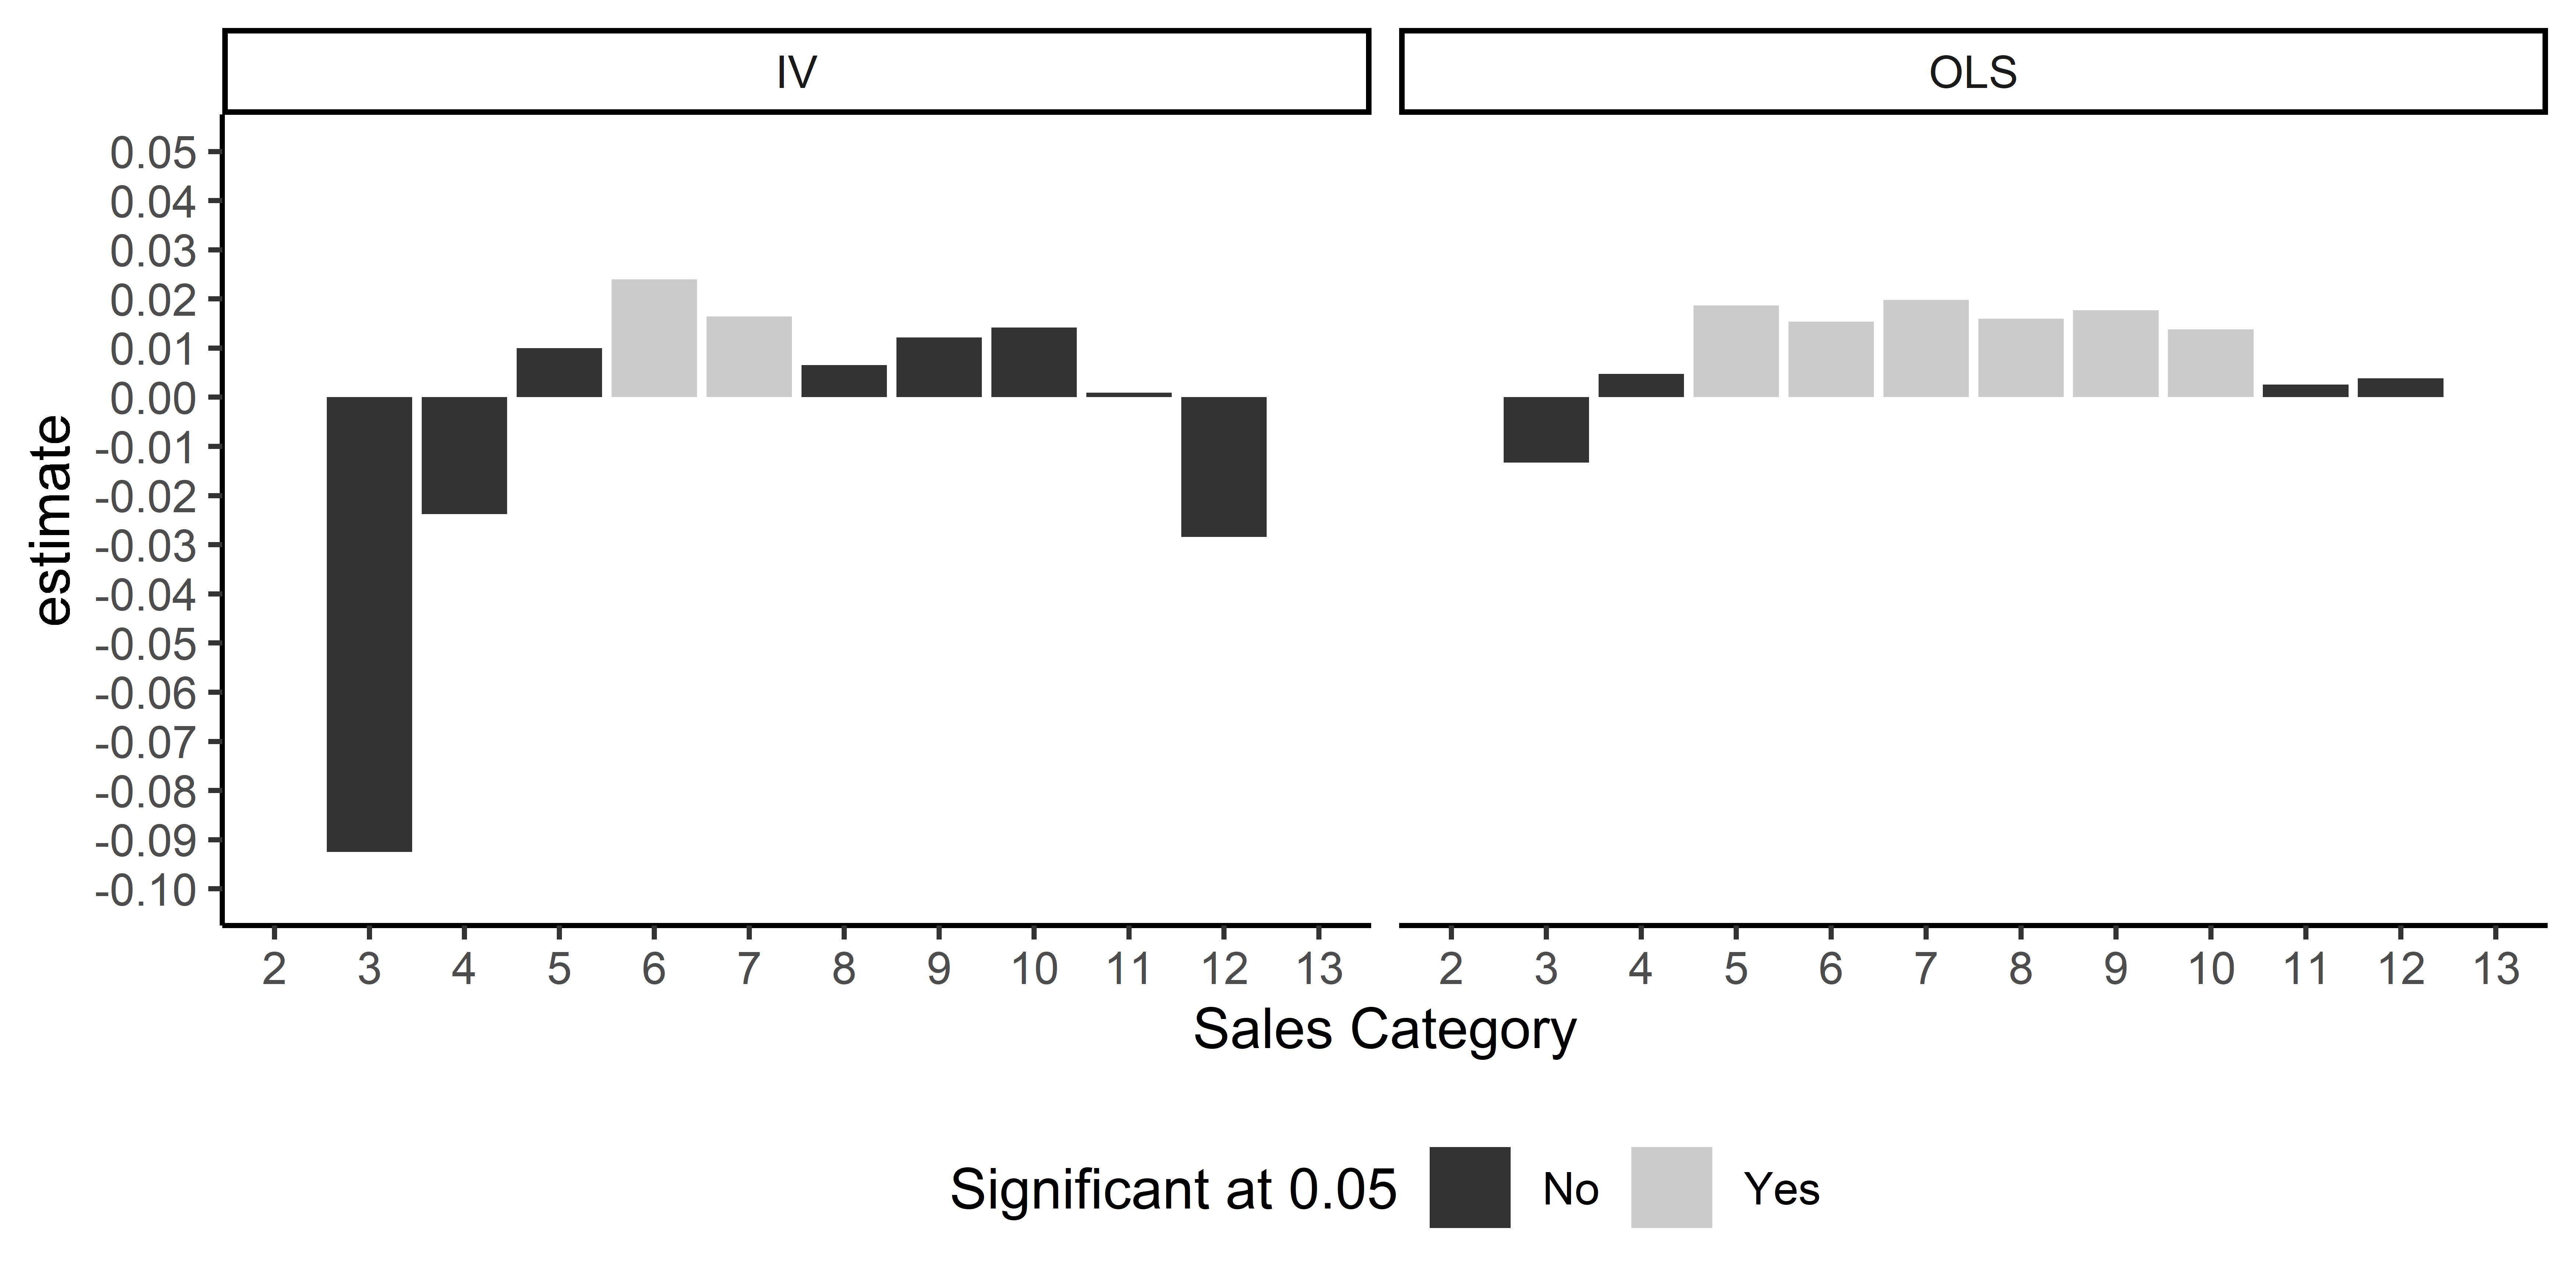
\includegraphics[scale=0.85]{plotsize.png}
%  \caption{Experience coefficient by tax sales category}
%  \label{fig:sizeestimates}
%\end{figure}


%\resizebox{\textwidth}{!}{%
%\input{C:/repos/learn-doing/thesis/tables/table_sizes_explinear1.txt}
%}%
\section{Robustness checks}
Several of our choices in the previous section admit several arbitrary choices. In this section we consider several extensions in parameters which could influence the results obtained before. We consider robustness checks in the following areas:

\subsection{Periods of outcomes}
In the previous section, we measured outcomes occuring in two year periods. We now consider outcomes occuring in one and three year periods as well. Note that in this part we only vary the length of the period where outcomes are computed and we maintain the procedure to compute experience as before. Table shows outcomes computed for periods of 1, 2(the original specifications) and 3 years. The first three columns employ the experience measured in the two-period previous to the outcome period while the 3-6 compute experience as annualized cumulative experience as discussed in the previous section.

\begin{table}[!htbp] \centering
\caption{Regression for OLS and IV specifications}
\label{}
\resizebox{\textwidth}{!}{%
\begin{tabular}{@{\extracolsep{5pt}}lcccccc}
\\[-1.8ex]\hline
\hline \\[-1.8ex]
& \multicolumn{6}{c}{Contracts Won/Contracts Bid in Outcome Period} \\
\cline{2-7}
\\[-1.8ex] & \multicolumn{6}{c}{Outcome period of length (years):} \\
& 1 & 2 (Original) & 3 & 1 & 2 (Original) & 3 \\
\hline \\[-1.8ex]
Experience & 0.022$^{***}$ & 0.020$^{***}$ & 0.023$^{***}$ &  &  &  \\
& (0.001) & (0.001) & (0.001) &  &  &  \\
& & & & & & \\
Annualized Cumulative Experience &  &  &  & 0.060$^{***}$ & 0.058$^{***}$ & 0.061$^{***}$ \\
&  &  &  & (0.002) & (0.002) & (0.002) \\
& & & & & & \\
Constant & 0.270$^{***}$ & 0.309$^{***}$ & 0.256$^{***}$ & 0.281$^{***}$ & 0.257$^{***}$ & 0.260$^{***}$ \\
& (0.005) & (0.005) & (0.004) & (0.005) & (0.007) & (0.004) \\
& & & & & & \\
\hline \\[-1.8ex]
Observations & 38,739 & 29,415 & 43,453 & 37,623 & 28,234 & 42,358 \\
R$^{2}$ & 0.028 & 0.031 & 0.025 & 0.026 & 0.028 & 0.023 \\
Residual Std. Error & 0.316 (df = 38730) & 0.338 (df = 29405) & 0.305 (df = 43445) & 0.320 (df = 37614) & 0.342 (df = 28224) & 0.309 (df = 42350) \\
\hline
\hline \\[-1.8ex]
\textit{Note:}  & \multicolumn{6}{r}{$^{*}$p$<$0.1; $^{**}$p$<$0.05; $^{***}$p$<$0.01} \\
\end{tabular}

}
\end{table}


\subsection{Periods of experience computation}
For the first measure of experience, we consider computing experience over 1-year periods. The original specification considered computing experience in two-year rolling periods.

In practice, considering longer periods to compute outcomes decreases the variance of th






%\item Different measures of experience: we consider time measures of experience instead of number of contracts won. We consider as the explanatory variab

\subsection{Definition of a close win}
In the previous section, we considered close wins as wins where the winning contractor submitted a bid that was not more than 0.05\% below the runner up. Now, we sensibilize our main coefficient to different values of this parameter.

 The plot in  \ref{fig:close_wins_robust} displays the coefficient of interest in the IV specification as we vary the threshold for a close win. The specifications consider linear effect of experience and fixed effects by period. It can be seen that results are robust to a range of the threshold for considering a win as a close wins. Note that the results remain significant across the different values of the parameters, even when  employ our lower bound for the threshold(0.01\%) where we have less close wins. As expected, the standard error increases towards this bound while but decreases towards  less stringent definitions of close wins (because of the increase in power in the instrument). Finally, note across that all confidence intervals at 95\% remain within 0.0180 and 0.0275.

 \begin{figure}[H]
         \centering
         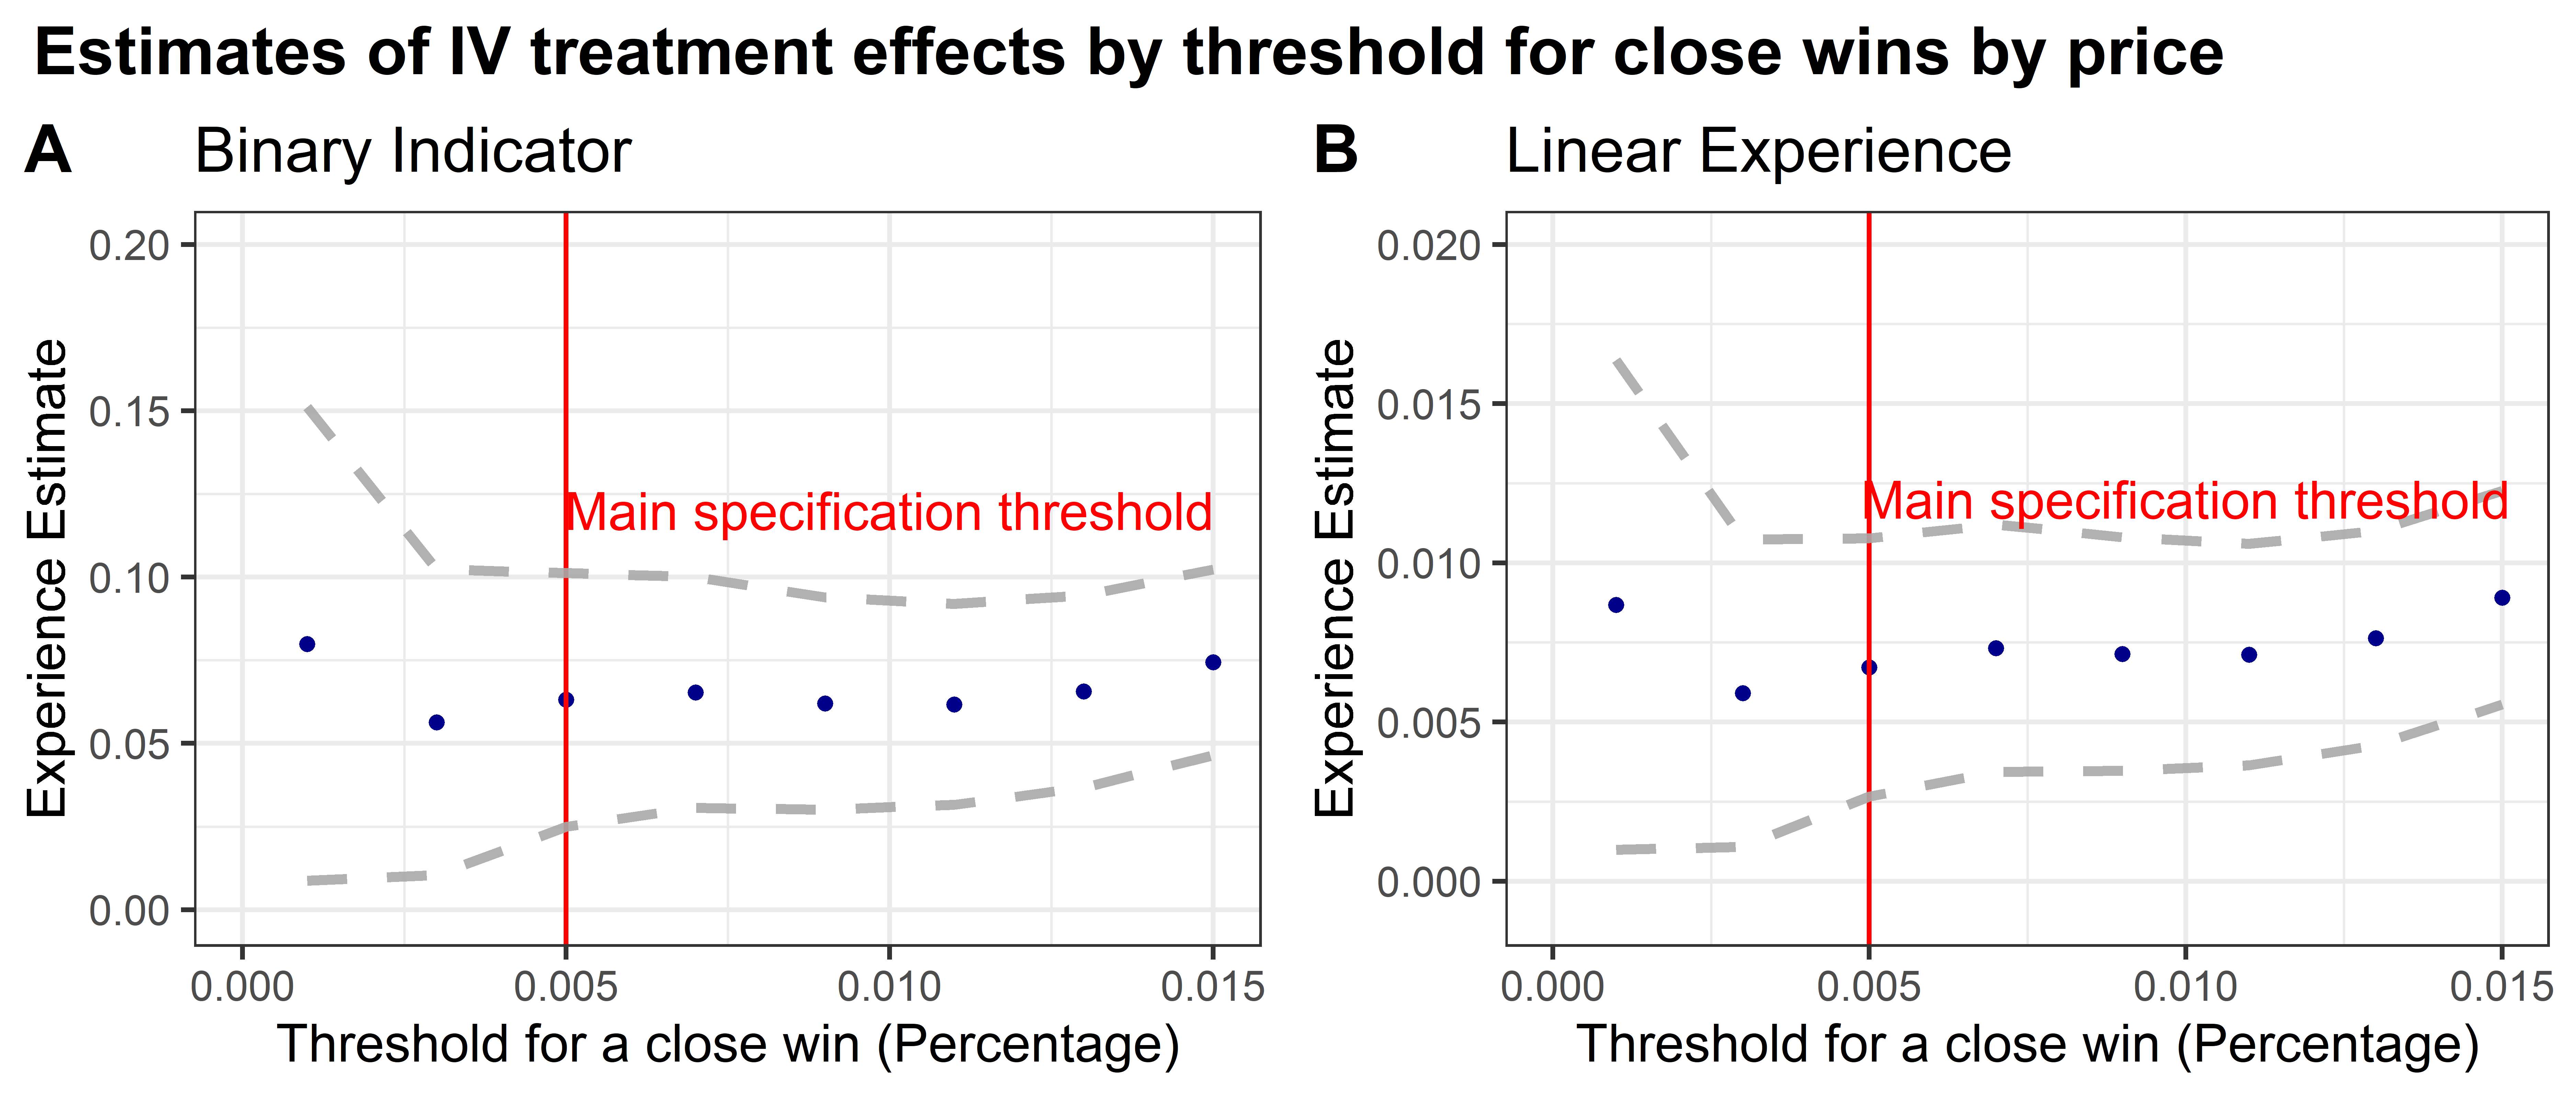
\includegraphics[scale=0.85]{robustness_threshold.png}
         \caption{Robustness analysis for threshold of close wins}
         \label{fig:close_wins_robust}

  \vskip 0.5mm
  {\justifying\footnotesize\underline{Note:} The plot shows the coefficient on experience as in the specification of Panel (5) of table \ref{tab:table_exp_1}, that is, the dependent variable is the share of contracts won in period $t$ and the dependent variable is linear experience, i.e. number of contracts won in period $(t-1)$, instrumented with close wins in period $(t-1)$. The $x$-axis shows how the coefficient varies with the threshold for what is considered a close win.\par}


     \end{figure}
